% titlepage-demo.tex
\documentclass[12pt]{beamer}
\usepackage{beamerthemesplit}
%\documentclass[notheorems]{beamer}
\usecolortheme[named=orange]{structure}
\usepackage[utf8]{vietnam}
\usepackage{listings}
\useoutertheme{infolines}
\usetheme[height=7mm]{Rochester}
%\usetheme{Copenhagen}
\usepackage{graphicx}
\usepackage{graphics,graphpap}
%\usetheme{CambridgeUS}
%\usetheme[height=7mm]{Madrid}
%\usetheme{CambridgeUS}
%\setbeamertemplate{items}[ball] 
% items enclosed in square brackets are optional; explanation below
%Thiết lập chế độ full màn hình khi mở slide
\hypersetup{pdfpagemode=FullScreen,
 bookmarks=false,unicode,bookmarksopen=false,unicode}
\title[Python \& công việc]{PYTHON \\ System / Network Administrator \\ DevOps}
\subtitle[PYTHONVIETNAM]{"Khơi dậy đam mê"}
%\author[tu0ng$\_$c0ng]{TÔ THÀNH CÔNG}
\author[Draft Version]{TÔ THÀNH CÔNG}
\institute[PYTHONVIETNAM.INFO]{
  Phòng Giải pháp \& Nghiên cứu phát triển\\
  Trung tâm công nghệ thông tin $@$ VDC \\
  http://vdc-it.vn\\[1ex]
  \texttt{tcvn1985@gmail.com}
}
\date{\today}
%Tạo ra đính lý và đánh số
\newtheorem{loihay}{Lời hay } 
\newtheorem{vidu}{Ví dụ}
\newcommand\Fontvi{\fontsize{6}{7.2}\selectfont} %Thiết lập kích thước font 
\newcommand\sFontvi{\fontsize{8}{7.2}\selectfont} %Thiết lập kích thước font 
%\newcommand\Fontvi2{\fontsize{8}{7.6}\selectfont} %Thiết lập kích thước font 
%Bắt đầu tài liệu
%% Gói lệnh highlighted source code
\lstnewenvironment{python}
{\lstset{language=python,
numbers=left,
xleftmargin=20pt,
keywordstyle={\color{blue}\ttfamily},
tabsize=3,
numberstyle={\tiny},
basicstyle={\ttfamily},
showspaces=false,
showstringspaces=false,
commentstyle= {\color{gray}}}}
{}
%%%%%%%%%%%%
\begin{document}
%--- the titlepage frame -------------------------%
\begin{frame}[plain]
  \titlepage
\end{frame}

%--- the presentation begin here -----------------%
\begin{frame}{Nội dung}
	\begin{enumerate}
 	 	\item tu0ng$\_$c0ng - WHO ?
  		\item Khi bạn nói ... mọi người nghĩ ...
  		%\item Tôi đã học gì và học như nào.
  		\item Python dành cho Network/System Administrator ..
  		\item Một số chương trình demo.
  		\item Tài nguyên \& tham khảo.
  		\item Trao đổi \& Thảo luận
  	\end{enumerate}  
\end{frame}
%--------------------------------------------------%
\label{Who}
\begin{frame}{1. Giới thiệu}
\sFontvi
\textit{\textit{Tô Thành Công}}\\
Đại học Thăng Long \\
Học viện NetPro (Sao Bắc Đẩu Academy)\\
Công ty Công Nghệ Việt | http://vtechco.com/ \\ 
Phòng tích hợp hệ thống | http://hsp-vn.com \\
\textbf{Hiện tại: Phòng giải pháp \& Nghiên cứu phát triển | http://vdc-it.vn }
\begin{figure}[!ht]
\centering
	\unitlength1cm
			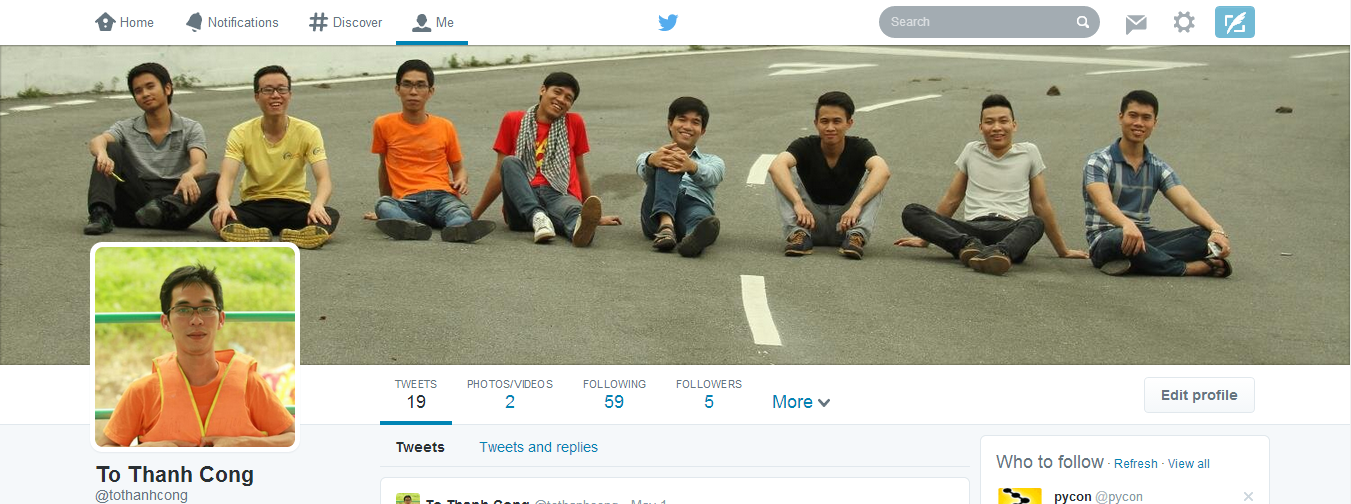
\includegraphics[scale=0.3]{congttwho}
\end{figure}
\end{frame}
%--------------------------------------------------%
\label{Khi toi noi}
\begin{frame}{2. Khi bạn nói ... mọi người nghĩ ...}
System Administrator / Network Administrator / System Monitor \\
Programmer / Coder / Tester / QA  \\
\textbf{DevOps ....}
\framebreak
\pause
\begin{figure}[!ht]
\centering
	\unitlength1cm
			
\includegraphics[scale=0.5]{khibannoi}
\end{figure}
%.......

%.......
\end{frame}
%--------------------------------------------------%
\label{Python & Cong viec}
\begin{frame}
\frametitle{3. Công việc của người quản trị hệ thống/mạng}
Triển khai / Vận hành / Hỗ trợ / Sao lư \& bảo trì / Nâng cấp \& cập nhật ...\\
%..........
\framebreak
\pause
\begin{figure}[!ht]
\centering
	\unitlength1cm
			
\includegraphics[scale=0.5]{automate-all-the-things}
\end{figure}
%..........
\end{frame}

%--------------------------------------------------%
\label{Python System netowrk OS}
\begin{frame}[fragile]
\frametitle{Python cho System / Network / (1) }
import os, sys, subprocess
\begin{block}{ipmort os}
\sFontvi
Cung cấp các "function" làm việc với hệ điều hành: Linux / Windows / MAC  \\
Bao gồm các việc: thực thi các lệnh / thông số trong hệ hiều hành ...
\framebreak
\pause
\end{block}
\begin{block}{Ví dụ về module OS} \label{Vi du ve module OS}
\Fontvi
\begin{python}
#!/use/bin/python
#
import os
print os.getcwd() 	#Hien thi duong dan hien tai
#os.system("tree") 	#Thu hien lenh ls trong Linux

#Tra ve thong tin cua file 
print "Getting the status of: ", os.stat('D:\Feedback cuoi ky.doc')

##Doi ten cua file	
print os.rename("D:\Feedback cuoi ky.doc", "D:\phanhoi.doc")

##Hien thi kich thuoc cua file - mac dinh theo bytes
print os.path.getsize("D:\phanhoi.doc")
\end{python}
\end{block}

\end{frame}

\begin{frame}[fragile]
\frametitle{Python cho System / Network / (2) }
\sFontvi
\begin{block}{Giới thiệu ipython}\label{Gioi thieu ipython}
Fabric is a Python (2.5-2.7) library and command-line tool for streamlining the use of SSH for application deployment or systems administration tasks.
\end{block}
ref:\\
http://www.pythonforbeginners.com/basics/ipython-a-short-introduction\\
http://ipython.org/documentation.html
\end{frame}
%------------------------------------
\begin{frame}{Python cho System / Network / (3) }
\sFontvi
\begin{block}{Giới thiệu về fabric} \label{fabric}
Fabric is a Python (2.5-2.7) library and command-line tool for streamlining the use of SSH for application deployment or systems administration tasks.
\end{block}
ref:\\
http://www.pythonforbeginners.com/fabric/how-to-use-fabric-in-python
\end{frame}
%--------------------------------------------------%
\label{Demo}
\begin{frame}[fragile] % Need to use the fragile option when verbatim is used in the slide
\frametitle{"Đề Mô"}
%%%%%%%%%%%%%%%%%%%%%%%%%%%%%%%%
\label{Chuong trinh scan port phan 1}
\begin{block}{Chương trình Scanport(1)}
\Fontvi
\begin{python}
#!/usr/bin/env python
#Source: http://www.pythonforbeginners.com/
import socket
import subprocess
import sys
from datetime import datetime

# Xoa man hinh trong LINUX
#subprocess.call("clear", shell=True)
# Xoa man hinh trong WINDOWS
subprocess.call("cls", shell=True)

# Nhap dia chi may chu
remoteServer    = raw_input("Nhap may chu can scan: ")
remoteServerIP  = socket.gethostbyname(remoteServer)

# Hien thi ra dong thong bao
print "-" * 60
print "Xin vui long doi, dang Scan may chu co dia chi", remoteServerIP
print "-" * 60

# Gan t1 bang thoi gian hien tai
t1 = datetime.now()
\end{python}
\end{block}
\end{frame}
%%%%%%%%%%%%%%%%%%%%%%%%%%%%%
\begin{frame}[fragile]
\begin{block}{Chương trình Scanport(2)}
\Fontvi
\begin{python}
#Scan tu port 1 den port 1024, dung try ... except de xu ly loi
try:
    for port in range(1,1025):  
        sock = socket.socket(socket.AF_INET, socket.SOCK_STREAM)
        result = sock.connect_ex((remoteServerIP, port))
        if result == 0:
            print "Port {}: \t Open".format(port)
        sock.close()

except KeyboardInterrupt:
    print "Ban da nhan Ctrl+C"
    sys.exit()

except socket.gaierror:
    print "Khong phan giai duoc ten mien, dang thoat ..."
    sys.exit()

except socket.error:
    print "Khong the ket noi den may chu"
    sys.exit()

# Gan thoi gian hien tai bang t2 (sau khi Scan)
t2 = datetime.now()
# Tong thoi gian Scan
total =  t2 - t1
# Hien thi ra man hinh
print "Tong thoi gian Scan la:", total
\end{python}
\end{block}
\end{frame}
%%%%%%%%%%%%%%%%%%%%%%%%%%%%%

%-------------------------------------------------%
\begin{frame}
\frametitle{Tài nguyên \& tham khảo.}
\framebreak
\pause
\textbf{Ebook}
\framebreak
\pause
\begin{itemize}
\item \textit{Python for Unix and Linux System Administration},\textbf{ Noah Gift, Jeremy M. Jones,} O'Reilly Media 2008.
\item \textit{Pro Python System Administration},\textbf{Rytis Sileika}, Apress 2010
\item \textit{Think Python How to Think Like a Computer Scientist},\textbf{Allen Downey}, Green Tea Press
\item \textit{A Byte of Python},\textbf{Swaroop C H}, swaroopch.com
\end{itemize}
%
\framebreak
\pause
\textbf{Cộng đồng \& website}
\framebreak
\pause
\begin{enumerate}
	\item http://pythonvietnam.info
	\item http://vithon.org
	\item http://stackoverflow.com/
	\item http://ipython.org/
	\item http://fabfile.org/
	\item http://sites.google.com/site/pythonforlinux/	
	\item http://pythonforbeginners.com/
	\item http://learnpythonthehardway.org/
\end{enumerate}
\end{frame}
%-------------------------------------------------%
\begin{frame}
\frametitle{Trao đổi \& thảo luận}
\Huge{\centerline{Cám ơn sự quan tâm của các bạn !}}
\sFontvi	
	\begin{itemize}
		\item Email: tcvn1985@gmail.com
		\item Twitter: http://twitter.com/tothanhcong
		\item Phone: 0912349490
	\end{itemize}
\end{frame}
%%%%%%%%%%%%%%%%%%%%%%%%%%%%%%%%%%%%%%%%%%%%%%%%%%%
\end{document}